\documentclass{standalone}
\usepackage{tikz}
\usetikzlibrary{patterns}
\usetikzlibrary{positioning}
\usetikzlibrary{patterns, positioning}
\usetikzlibrary{shapes.misc}
\usepackage[outline]{contour}
\contourlength{1.5pt} 
\usepackage[sfdefault]{ClearSans}

\begin{document}
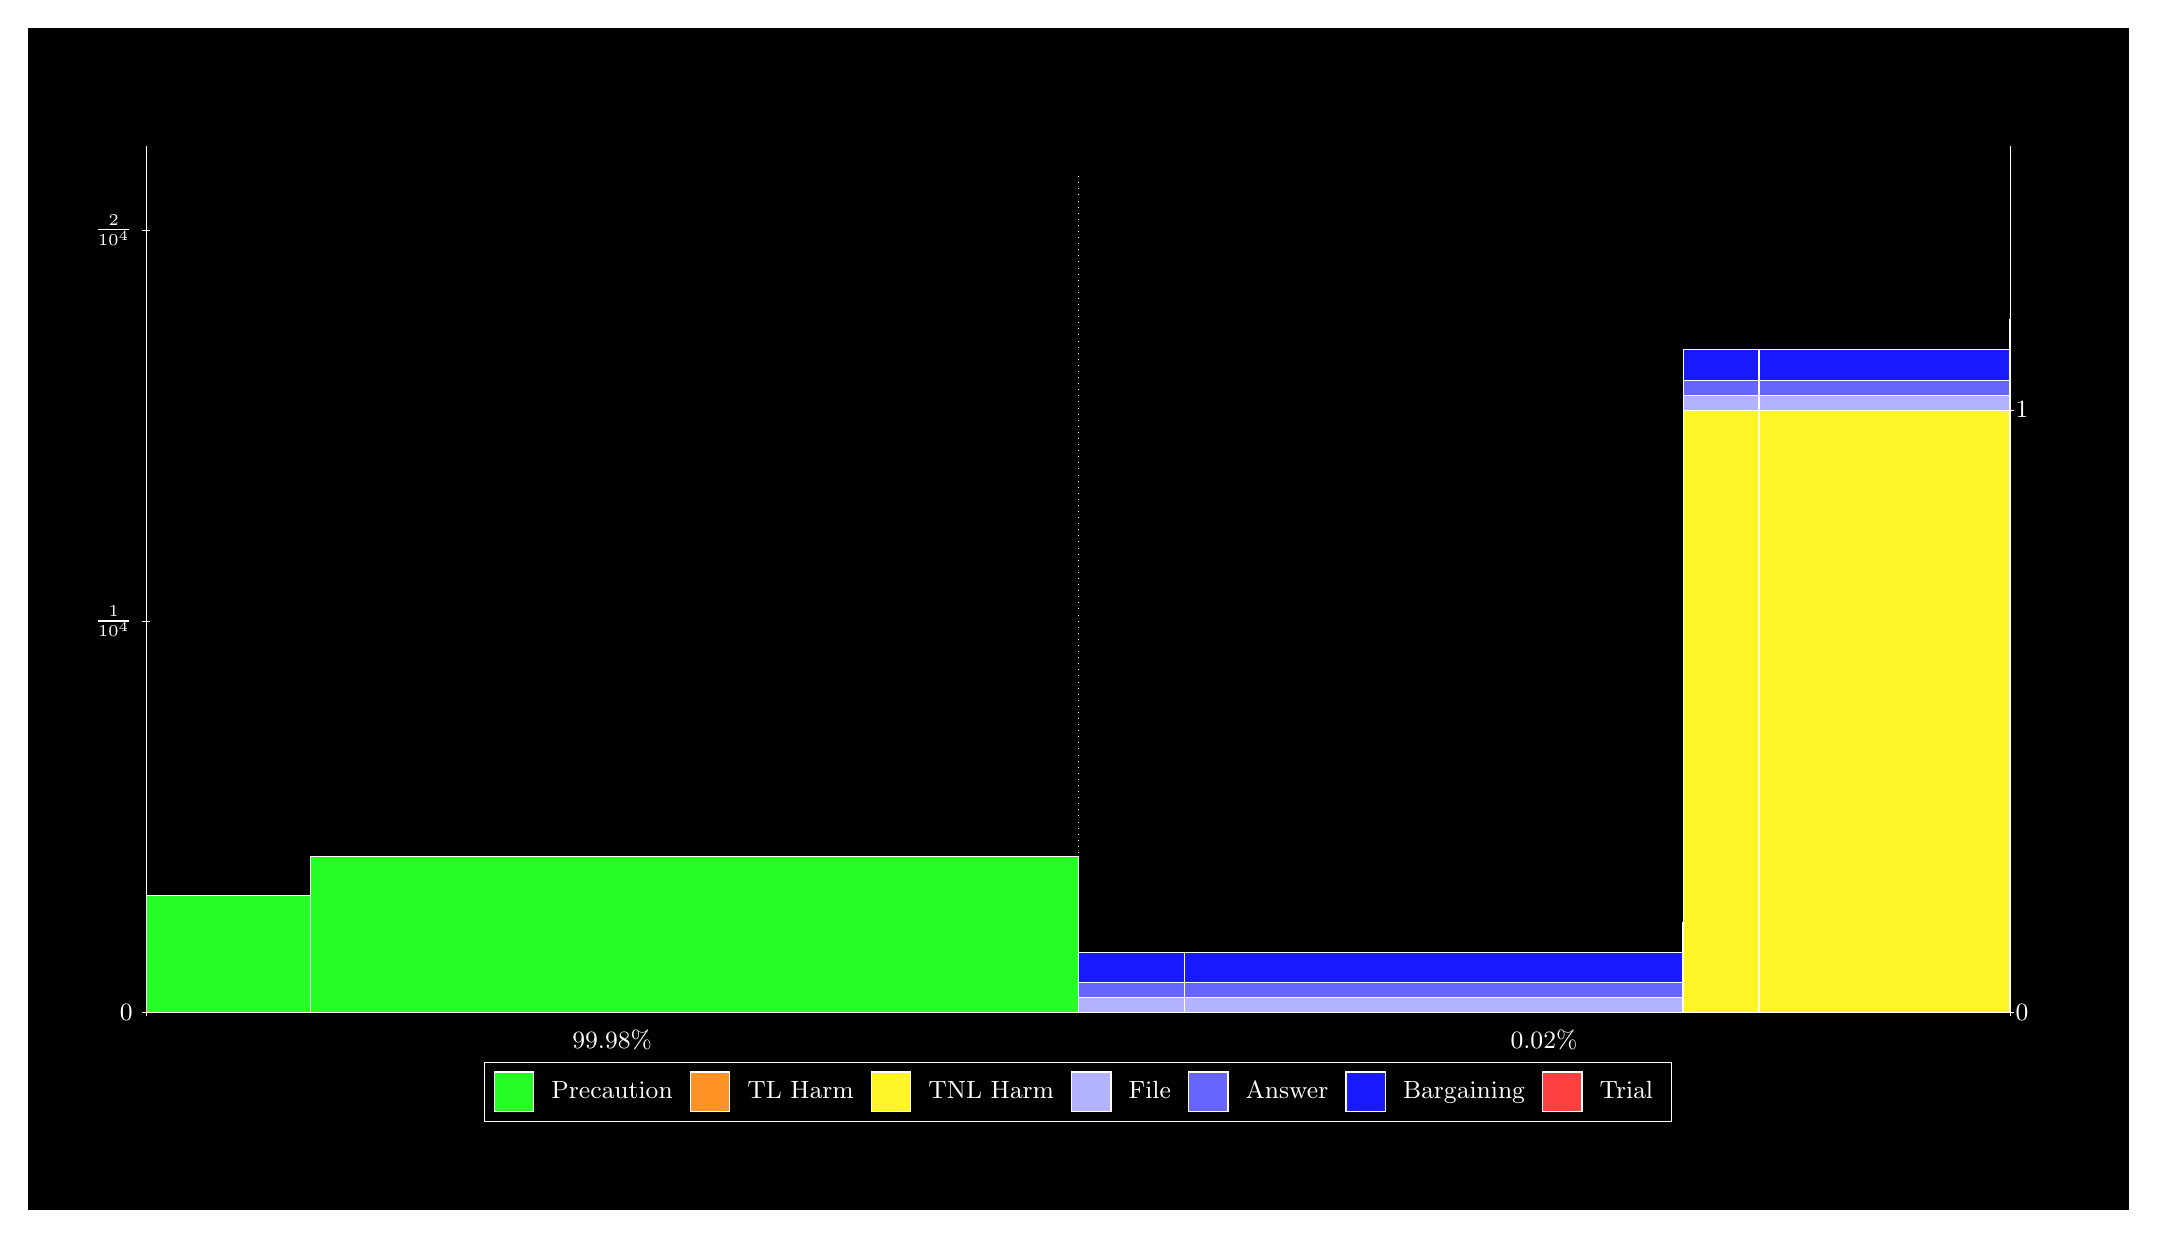
\begin{tikzpicture}
\draw[fill=black] (0,0) rectangle (26.667,15);
\draw[fill=green!85,draw=white,very thin] (1.5,2.5) rectangle (3.585,3.9904);
\draw[fill=green!85,draw=white,very thin] (3.585,2.5) rectangle (13.333,4.4872);
\draw[fill=green!85,draw=white,very thin] (13.333,2.5) rectangle (14.676,2.5002);
\draw[fill=blue!30,draw=white,very thin] (13.333,2.5002) rectangle (14.676,2.6915);
\draw[fill=blue!60,draw=white,very thin] (13.333,2.6915) rectangle (14.676,2.8828);
\draw[fill=blue!90,draw=white,very thin] (13.333,2.8828) rectangle (14.676,3.2654);
\draw[fill=green!85,draw=white,very thin] (14.676,2.5) rectangle (21.005,2.5003);
\draw[fill=blue!30,draw=white,very thin] (14.676,2.5003) rectangle (21.005,2.6916);
\draw[fill=blue!60,draw=white,very thin] (14.676,2.6916) rectangle (21.005,2.8829);
\draw[fill=blue!90,draw=white,very thin] (14.676,2.8829) rectangle (21.005,3.2655);
\draw[fill=green!85,draw=white,very thin] (21.005,2.5) rectangle (21.017,2.5002);
\draw[fill=blue!30,draw=white,very thin] (21.005,2.5002) rectangle (21.017,2.6915);
\draw[fill=blue!60,draw=white,very thin] (21.005,2.6915) rectangle (21.017,2.8828);
\draw[fill=blue!90,draw=white,very thin] (21.005,2.8828) rectangle (21.017,3.2654);
\draw[fill=red!75,draw=white,very thin] (21.005,3.2654) rectangle (21.017,3.648);
\draw[fill=green!85,draw=white,very thin] (21.017,2.5) rectangle (21.977,2.5002);
\draw[fill=yellow!85,draw=white,very thin] (21.017,2.5002) rectangle (21.977,10.152);
\draw[fill=blue!30,draw=white,very thin] (21.017,10.152) rectangle (21.977,10.344);
\draw[fill=blue!60,draw=white,very thin] (21.017,10.344) rectangle (21.977,10.535);
\draw[fill=blue!90,draw=white,very thin] (21.017,10.535) rectangle (21.977,10.917);
\draw[fill=green!85,draw=white,very thin] (21.977,2.5) rectangle (21.98,2.5002);
\draw[fill=orange!85,draw=white,very thin] (21.977,2.5002) rectangle (21.98,10.152);
\draw[fill=blue!30,draw=white,very thin] (21.977,10.152) rectangle (21.98,10.344);
\draw[fill=blue!60,draw=white,very thin] (21.977,10.344) rectangle (21.98,10.535);
\draw[fill=blue!90,draw=white,very thin] (21.977,10.535) rectangle (21.98,10.917);
\draw[fill=green!85,draw=white,very thin] (21.98,2.5) rectangle (25.16,2.5003);
\draw[fill=yellow!85,draw=white,very thin] (21.98,2.5003) rectangle (25.16,10.152);
\draw[fill=blue!30,draw=white,very thin] (21.98,10.152) rectangle (25.16,10.344);
\draw[fill=blue!60,draw=white,very thin] (21.98,10.344) rectangle (25.16,10.535);
\draw[fill=blue!90,draw=white,very thin] (21.98,10.535) rectangle (25.16,10.917);
\draw[fill=green!85,draw=white,very thin] (25.16,2.5) rectangle (25.165,2.5002);
\draw[fill=yellow!85,draw=white,very thin] (25.16,2.5002) rectangle (25.165,10.152);
\draw[fill=blue!30,draw=white,very thin] (25.16,10.152) rectangle (25.165,10.344);
\draw[fill=blue!60,draw=white,very thin] (25.16,10.344) rectangle (25.165,10.535);
\draw[fill=blue!90,draw=white,very thin] (25.16,10.535) rectangle (25.165,10.917);
\draw[fill=red!75,draw=white,very thin] (25.16,10.917) rectangle (25.165,11.3);
\draw[fill=green!85,draw=white,very thin] (25.165,2.5) rectangle (25.167,2.5002);
\draw[fill=orange!85,draw=white,very thin] (25.165,2.5002) rectangle (25.167,10.152);
\draw[fill=blue!30,draw=white,very thin] (25.165,10.152) rectangle (25.167,10.344);
\draw[fill=blue!60,draw=white,very thin] (25.165,10.344) rectangle (25.167,10.535);
\draw[fill=blue!90,draw=white,very thin] (25.165,10.535) rectangle (25.167,10.917);
\draw[fill=red!75,draw=white,very thin] (25.165,10.917) rectangle (25.167,11.3);
\draw[white,very thin] (1.5,2.5) -- (1.5,13.5);
\draw[white,very thin] (1.45,2.5) -- (1.55,2.5);
\node[font=\small,text=white, anchor=east] at (1.45, 2.5) {0};
\draw[white,very thin] (1.45,7.468) -- (1.55,7.468);
\node[font=\small,text=white, anchor=east] at (1.45, 7.468) {$\frac{1}{10^{4}}$};
\draw[white,very thin] (1.45,12.436) -- (1.55,12.436);
\node[font=\small,text=white, anchor=east] at (1.45, 12.436) {$\frac{2}{10^{4}}$};

\draw[white,dotted,very thin] (13.333,2.83) -- (13.333,13.17);
\draw[white,very thin] (25.167,2.5) -- (25.167,13.5);
\draw[white,very thin] (25.117,2.5) -- (25.217,2.5);
\node[font=\small,text=white, anchor=west] at (25.117, 2.5) {0};
\draw[white,very thin] (25.117,10.152) -- (25.217,10.152);
\node[font=\small,text=white, anchor=west] at (25.117, 10.152) {1};

\draw[white,very thin] (1.5,2.5) -- (25.167,2.5);
\draw[white,very thin] (1.5,2.45) -- (1.5,2.55);
\node[font=\small,text=white, anchor=north] at (1.5, 2.45) {};
\draw[white,very thin] (25.167,2.45) -- (25.167,2.55);
\node[font=\small,text=white, anchor=north] at (25.167, 2.45) {};

\node[font=\small,text=white,anchor=south] at (7.4167, 1.9) {99.98\%};
\node[font=\small,text=white,anchor=south] at (19.25, 1.9) {0.02\%};
\draw (13.3333,2.5) node (B) {};
\begin{scope}[align=center]
\matrix[scale=0.5,draw=white,below=0.5cm of B,nodes={draw},column sep=0.1cm]{
\node[rectangle,draw,minimum width=0.5cm,minimum height=0.5cm,fill=green!85]{}; & \node[draw=none,font=\small,text=white]{Precaution}; &
\node[rectangle,draw,minimum width=0.5cm,minimum height=0.5cm,fill=orange!85]{}; & \node[draw=none,font=\small,text=white]{TL Harm}; &
\node[rectangle,draw,minimum width=0.5cm,minimum height=0.5cm,fill=yellow!85]{}; & \node[draw=none,font=\small,text=white]{TNL Harm}; &
\node[rectangle,draw,minimum width=0.5cm,minimum height=0.5cm,fill=blue!30]{}; & \node[draw=none,font=\small,text=white]{File}; &
\node[rectangle,draw,minimum width=0.5cm,minimum height=0.5cm,fill=blue!60]{}; & \node[draw=none,font=\small,text=white]{Answer}; &
\node[rectangle,draw,minimum width=0.5cm,minimum height=0.5cm,fill=blue!90]{}; & \node[draw=none,font=\small,text=white]{Bargaining}; &
\node[rectangle,draw,minimum width=0.5cm,minimum height=0.5cm,fill=red!75]{}; & \node[draw=none,font=\small,text=white]{Trial}; \\\\
};\end{scope}

\end{tikzpicture}
\end{document}